\documentclass[10.5pt, a4paper, twoside]{article}
\providecommand{\abs}[1]{\lvert#1\rvert}
\setlength{\topmargin}{-1.25in}
\setlength{\footskip}{0.75in}
\setlength{\textheight}{10in}

\usepackage[margin=2.5cm]{geometry}
\usepackage{amsfonts}
\usepackage{amsmath}
\usepackage{amssymb}
\usepackage{graphicx}
\usepackage{enumerate}
\usepackage{color}
\usepackage{float}
\usepackage{multirow}
\usepackage{setspace}
\usepackage{tabularx}
\setlength{\extrarowheight}{5pt}
\usepackage[labelfont=bf]{caption}
\usepackage{subfig}
\usepackage[bookmarks]{hyperref} % Creates index and hyperlinks
\usepackage[T1]{fontenc} % Don't get confused by | < >

\usepackage{perpage}
\MakePerPage{footnote}

%%%% BIBLIO

\usepackage[backend=bibtex]{biblatex}

%%%% GLOSSARY STUFF

\usepackage[intoc]{nomencl}

\renewcommand{\nomname}{Glossary}
\renewcommand{\nomlabel}[1]{\textbf{#1}}
\makenomenclature

%\singlespacing
\onehalfspacing
%\doublespacing
%\setstretch{1.1}

\setlength\parindent{0pt}

\newenvironment{packed_itemize}{
\begin{itemize}
  \setlength{\itemsep}{1pt}
  \setlength{\parskip}{0pt}
  \setlength{\parsep}{0pt}
}{\end{itemize}}

\definecolor{dkgreen}{rgb}{0,0.6,0}
\definecolor{gray}{rgb}{0.5,0.5,0.5}
\definecolor{mauve}{rgb}{0.58,0,0.82}

\newcommand{\vecthree}[3]{\left(\!\!{\scriptsize\begin{array}{c}#1\\#2\\#3\end{array}}\!\!\right)}
\newcommand{\vectwo}[3]{\left(\!\!{\scriptsize\begin{array}{c}#1\\#2\end{array}}\!\!\right)}
\newcommand{\HRule}{\rule{\linewidth}{0.5mm}}

\newcommand{\ggather}[1]{\begin{gather}#1\end{gather}}
\newcommand{\nggather}[1]{\begin{gather}#1\end{gather}}

\newcolumntype{C}{>{\centering\arraybackslash}X}
\newcolumntype{L}{>{\raggedright\arraybackslash}X}

\addbibresource{sources.bib}

\begin{document}
%
%\title{ \bf \huge Development of a 12.4 GHz Bandwidth Frequency Offset Locking Unit for Two-Laser Systems}
%\author{Steve Novakov }
%\date{}
%
%\maketitle

\begin{titlepage}
\begin{center}

% Upper part of the page. The '~' is needed because \\
% only works if a paragraph has started.

% Title
\HRule \\[0.4cm]
{ \huge \bfseries Pound-Drever-Hall Servomechanism with an Atomic Gas Reference for Frequency Stabilization of a Master Laser \\[0.4cm] }

\HRule \\[1.3cm]

{ \huge \bfseries Final Recommendation Report \\[1.3cm] }

% Author and supervisor

\begin{tabularx}{\linewidth}{lXr}
  \Large \emph{Authors:} & & \Large \emph{Sponsor:} \\
  \Large \textsc{Steve Novakov} & & \Large \textsc{Dr.~Kirk Madison} \\
  \Large \textsc{Jeff Taylor}  & & \\
\end{tabularx}

\vfill

\textsc{\LARGE ENPH 479}\\[0.3cm]
\textsc{\LARGE Engineering Physics}\\[0.3cm]
\textsc{\LARGE University of British Columbia}\\[0.3cm]

\vfill

\textsc{\Large Group 1472}\\[0.3cm]
\textsc{\Large Project 33}\\[0.3cm]

\vfill

% Bottom of the page
{\large \today}

\end{center}
\end{titlepage}
\newpage

%%%%%%%%%%%%%%%% EXECUTIVE SUMMARY

\newpage
\section*{Executive Summary}

This project, sponsored by Dr. Kirk Madison of the UBC Quantum Degenerate Gases Laboratory, invovled the construction and characterization of a robust laser frequency locking system based on the Pound-Drever-Hall locking method. \\

Existing systems at the sponsors' laboratory are already based on the PDH method, but use a slightly different approach.  Both the existing and proposed systems lock to a vapour cell.  The existing locking unit uses an acousto-optic modulator, which uses acoustics to produce a frequency-shifted diffraction pattern.  This pattern is filtered through a vapour cell, and then coupled into a photosensor.  From there, frequency-shifted parts are extracted, which produces an error signal.  This error signal locks the diode laser's control system to the desired transition resonance. The existing system is severaly limited in that the error signal has poor stability, low bandwidth, and is subject to various modulation effects which change the location of its null locking points. \\

The new, EOM based, feedback system built here addresses these issues and hints at further improvements. A table-based optical setup based around modulation transfer spectroscopy was constructed and a Pound-Drever-Hall type error signal was generated using a photosensor and discrete RF components. The resulting signal has improved stability and non-drifting locking points. The resulting SNR is worse in the new system by a factor of two due to suboptimal component choices. However, simple change to more robust, readily available, electrical components will improve this by a factor of four, at minimum. \\

Closed loop testing to determine linewidth and carrier stability improvements was not possible due to time constraints, difficulty, and equipment availability. The sponsor was supplied with a full set of characterization data to specify the optimal configuration and is well poised to reconstruct this system on their main optical table at their convenience.



%%%%%%%%%%%%%%%% TOC / FIGURES / TABLES
\newpage
\tableofcontents
\newpage
\listoffigures
\listoftables

%%%%%%%%%%%%%%% GLOSSARY

\newpage
\section*{Glossary}

\begin{tabularx}{\linewidth}{lX}
  {\bf AOM} & Acousto-optic modulator: a device which uses acoustic waves to vary the direction of a light beam, and in turn the distance it must travel, creating a doppler-shifted diffraction pattern. \\
  {\bf AM/FM} & Amplitude modulation and frequency modulation. \\
  {\bf CCA} & Circuit Card Assembly: includes a PBC and all of its components,
  sometimes encludes complimentary mechanical components as well. \\
  {\bf FWHM} & Full width half maximum, a measure of width of a Gaussian or Lorentzian like feature. \\
  {\bf ECDL} & External cavity diode laser. \\
  {\bf EOM} & Electro-optic modulator: also known as a Pockels cell, this
  is an optical medium which is subject to the Pockels effect: electrically
  modulating the phase of an incident electromagnetic wave in the direction
  of propagation.\\
  {\bf EMI} & Electromagnetic Interference: two types: radiated and conducted.\\
  {\bf FO (Receiver)} & Fiber Optic (photosensor unit for detecting fiber optic
  signals).  \\
  {\bf L/H/BPF} & Low-pass, High-pass, and Band-Pass Filter, respectively. \\
  {\bf PCB} & Printed Circuit Board. \\
  {\bf PDH} & Pound-Drever-Hall. Refers to a method of generating an RF signal to resolve a frequency selective feature from higher frequency optical signals. \\
  {\bf Pol Cube} & A polarization cube.  Filters light such that horizontally polarized light passes straight through, and vertically polarized light reflects. \\
  {\bf RF} & Radio Frequency. Used to refer to components or systems which
  operate in the 3 kHz - 300 GHz regime. \\
  {\bf SNR} & Signal-to-noise ratio. Roughly, this is the ratio of the maximum signal amplitude to the amplitude of constant background noise. \\
  {\bf VCO} & Voltage Controlled Oscillator, may be crystal or PLL based. \\
  {\bf $V_{PP}$} & Peak-to-peak voltage: the full range of voltage of a
  particular waveform.
\end{tabularx}


%%%%%%%%%%%%%%%% BACKGROUND/MOTIVATION/OBJECTIVES

\newpage
\section{Introduction}

The ability to lock a laser to a very specific frequency is of great importance to the UBC Quantum Degenerate Gases Laboratory.  They use these optical systems to laser cool atomic and molecular gases.  This requires a very narrow laser linewidth, and a stable carrier frequency.  Any improvement in the frequency precision of the laser will increase the quantity of atoms that can be trapped or cooled, as well as the attainable temperatures in a trap.  Often, this frequency must be very close to the natural transitions of the gas. \\

One way to acquire such a system is to pass the beam through a gas.  The gas has state transitions at particular optical frequencies, which can be detected by sweeping the probing laser. The gas will absorb photons most strongly at the atomic transition resonances, which will appear as sharp dips in the transmission spectrum.  However, since the gas is at room temperature, the broad absorption dip will have a bandwidth of about 1 GHz, which is too wide for accurate laser locking.

The Madison group has an existing system to lock lasers to various atomic transitions using AOM-based saturated absorption spectroscopy and the Pound-Drever-Hall method. However, this system is limited in a number of ways: \\
\begin{tabularx}{\linewidth}{lX}
  Stability & Currently, the signal is processed in a way that leaves it sensitive to acoustic perturbations. As such, it has a large jitter amplitude during operation, which results in higher laser linewidths and, occasionally, total loss of locking. \\
  Bandwidth & Due to the low bandwidth of various components (including the modulating element) the signal's bandwidth is limited to approximately 10 kHz. This reduces the speed at which the laser servo can acquire a lock. \\
  Zero Crossings & Due to AM pickup, shifts of alignment and laser power, the null locking points actually shift around during operation. As stated, shifts away from precise atomic transitions reduce the efficiency of experiments.
\end{tabularx} \\ \ \\
This project aims to improve various elements of this feedback system to improve stability, bandwidth and SNR and minimize the need for manual tuning. Furthermore, the methods employed here remove DC shifts in the error signal zero crossings. These improvements will lead to a master laser that has smaller linewidth and a more accurate/stable carrier frequency.

\subsection{Doppler Effects}

The gas in a vapour cell is at room temperature. In a saturated absorption spectroscopy scheme, for example, some atoms will be moving towards the probe beam, and other atoms will be moving away from it. As a result, if a single laser is used, the atoms moving towards the laser will perceive a higher frequency, and thus will excite at lower frequencies than the resonance frequency.  The opposite is also true.  If the absorption-vs-frequency curve is measured for a laser passed through the gas, there is a wide smear that is approximately 1 GHz wide \cite{madison14}.  This makes the apparent spectrum of the gas much wider, and thus, much harder to lock a signal to. This is depicted in \textbf{Figure \ref{fig:doppler}}. \\

A major improvement is to redirect the single frequency laser around the sample, to the opposite side.  Now, when the sweep laser is at the same frequency as the pumping laser, its light will not be absorbed by the atoms with zero horizontal velocity.  This creates a Doppler-cancelled feature, which is about 10--100MHz wide.

\subsection{Acousto-Optic Modulator}

One way to modulate the frequency of the beam is to use an acousto-optic modulator (AOM). An AOM is a device that acoustically varies its shape, adjusting the distance the light has to travel to reach its destination.  By driving the optical medium at a particular frequency, an incident beam of light is diffracted and Doppler shifted depending on what angle it is sampled at. Modulating this driving frequency at an additional frequency $\Omega$, produces a beam of light that is phase modulated at a frequency $\Omega$. \\

AOMs are limited by the mechanical properties of the optical medium. Specifically, while being driven at some nominal frequency that may reach up to 100s of MHz, they can only register a frequency modulation at a rate up to several MHz. This is due to the fact that the rate of acoustic propagation across the medium is limited. Depending on what refraction angle it is sampled at, the output beam of the acousto-optic modulator also contains a shift in the carrier frequency.  This shift needs to be accounted for in a later stage of the system.

\subsection{Electro-Optic Modulator}

An \emph{electro-optic modulator} (EOM), is a device that uses an electric field to modulate the phase of an EM wave.  These devices exploit the effects of strong nonlinear susceptibility, whereby the speed of light in a crystal is affected by the presence of an electric field.  Therefore, by adjusting the electric field in the crystal, the phase (and ultimately frequency spectrum) of the beam can be varied. The EOM does \emph{not} shift the carrier frequency, unlike an AOM. Furthermore, the resultant phase modulation frequency of the incident laser can reach into the GHz range, orders of magnitude above the
capability of an AOM.\\

Unfortunately, the EOM requires fairly large driving voltages, on the order of hundreds of volts.  Some manufacturers provide a full EOM solution, with built-in amplifier, to make their equipment easier to use, making an external high-voltage amplifier unnecessary. This project makes use of a homebuilt EOM/driver system based around a Lithium Niobiate (LiNbO$_3$) crystal.

\subsection{The Pound-Drever-Hall Method}

Optical frequencies generally exceed 100THz. It is not possible to extract information at these frequencies using conventional electronic measurement equipment. Systems make use of schemes that down-mix these optical signals into RF range, which are then processed via conventional means (RF electronics and digital systems). \\

The Pound-Drever-Hall method makes use of phase-modulated light to measure an optical response and down-mix it into RF range.  This signal is then mixed again with the same oscillator to produce a DC signal. Changing the modulation frequency varies the resolution of this derivative function. At extremes, this derivative function is either small and featureless, or is excessively noisy and not useful. \\

This method is used to lock to extrema of absorption spectra.  In an atomic gas, these features are typically transition and crossover resonances \cite{maguire2006}. Carefully selecting a modulation frequency to obtain a useful error signal about a point of interest is a principal challenge of implementing this method.

\subsection{Spectroscopy Methods}

There are a variety of methods to generate an absorption spectrum from an atomic gas, involving different configurations of cell/beam alignment, beam power ratios and various signal processing techniques. The original proposal involved the use of saturated absorption spectroscopy, which is elaborated on in \textbf{Section \ref{sec:sat_abs}}. However, due to various parasitic effects and poor SNR, (see \textbf{Figure \ref{fig:sat_abs_bad}}) the final configuration made use of a modulation transfer scheme, which has been described well in the literature \cite{Shirley:82}. There have also been detailed experiments specifically involving Rubidium, which were a good starting point for this project \cite{0957-0233-19-10-105601}. These processes are described in more detail in \textbf{Section \ref{sec:theory}}.

\begin{figure}
    \centering
    \includegraphics[width=0.45\textwidth]{figures/doppler.png}
    \caption{Doppler effect demonstration.  The probe beam is absorbed across a wide frequency range, but only the non-Doppler-shifted particles are affected by both beams from left and right.}
    \label{fig:doppler}
\end{figure}

\begin{figure}
  \begin{tabular}{cc}
    \includegraphics[width=0.47\textwidth]{figures/{AOM_85}.png} &
    \includegraphics[width=0.47\textwidth]{figures/{AOM_87}.png} \\
  \end{tabular}
  \caption{Existing AOM-based, single demodulation channel error signals around Rb85 (left) and Rb87 (right) D2 transitions. Each figure shows the reference spectrum (black), and the resulting PDH error signal (red).}
  \label{fig:aom_spectra}
\end{figure}

\begin{figure}
    \centering
    \includegraphics[width=0.5\textwidth]{figures/best_sat_abs.png}
    \caption{Saturated absorption spectroscopy based PDH signal acquired near the start of the project. Shown is the ramping signal (yellow), AOM-based reference saturated absorption spectrum (blue) and the new EOM-based PDH signal (pink). This signal is suboptimal due to low SNR (approximately 3:1), which was difficult to improve given avai,lable resources. Additionaly, AM pickup effects bring into question the accuracy of the zero crossings.}
    \label{fig:sat_abs_bad}
\end{figure}


%%%%%%%%%%%%%%%% BACKGROUND THEORY

\newpage
\section{Theory}
\label{sec:theory}

To gain an understanding of the motivations behind this project it is worthwhile to discuss both prior work done with the PDH method, and the motivations behind using it to lock to an atomic source.  The PDH method is often used to lock a laser to a reference cavity \cite{black1998}.  The Madison group primarily performs laser cooling experiments on Lithium and Rubidium gas.  They need to precisely set laser frequencies at or near key atomic transitions. This project focuses on the Rb87 and Rb85 $5S_{1/2} \rightarrow 5P_{3/2}$ transitions, specifically Rb87 $\left|F=2\right\rangle \rightarrow F'$ and Rb85 $\left|F=3\right\rangle \rightarrow F'$.  The closer a laser's frequency is to a desired transition and the smaller the linewidth of that laser, the more efficient any excitation will be.  This efficiency has a direct impact on experimental outcome.

%%%%%%%%%%%%%%%%%%%%%%%%%%%%%%%%%%%%%%%%%%%%%%%%%%%%%%%%%%%
%%%%%%%%    Phase Modulation
%%%%%%%%%%%%%%%%%%%%%%%%%%%%%%%%%%%%%%%%%%%%%%%%%%%%%%%%%%%

\subsection{Optical Phase Modulation}

Phase modulation of optical signals is typically achieved with either an AOM or an EOM. From a practical standpoint, the main difference between the two methods is what phase modulation depths and frequencies are physically attainable. \\

With an AOM which use acoustic waves to Doppler shift a beam in the transverse direction of propagation, there is a distinct tradeoff between modulation frequency and the resultant power of the outgoing beam.  The AOM units currently used by the Madison Group only have a useful modulation frequency of $\sim$200 kHz \cite{madison14}. \\

The modulation frequency of an EOM is sustainable well into the 100 MHz range, with modulation depth a function of the driving voltage. Furthermore, as phase modulation is parallel with the beam propagation, there is no significant decrease in total beam power as the modulation frequency is increased. Typical modulation depths are in the 100mRad range, with a driving voltage of $\sim 10 V_{pp}$ \cite{thorlabs_eom}. A larger modulation depth demands a higher driving voltage. \\

The effect of the phase modulating medium is to induce a phase oscillation in the incident laser:
\begin{gather}
  E = E_0 e^{i\omega t} \xrightarrow{\mbox{Phase Modulation}}
    E_0 e^{i \omega t + \beta \sin \Omega t}
\end{gather}
where $\beta$ is defined as the modulation depth, in radians, and $\Omega$ is the modulation frequency. Using the Jacobi-Anger expansion to isolate the sideband amplitudes,

\begin{gather}
  E_0 e^{i \omega t + \beta \sin \Omega t}  =
  E_0 e^{i\omega t} \sum_{n = -\infty}^{n = \infty} J_n(\beta)e^{in\Omega}
\end{gather}

it is shown that a sideband of frequency $(\omega +n\Omega)$ has amplitude $J_n(\beta)$, the Bessel function of order $n$, evaluated at $\beta$. In this implementation, the sideband power is approximately 14\% of the carrier's.

\begin{figure}
  \centering
  \includegraphics[width=0.6\textwidth]{figures/spectrum.png}
  \caption{Expected spectrum of beam after EOM phase modulation, to the first
  sidebands. While possibly present and significant, further sidebands can
  be ignored as they will be filtered during mixing.}
  \label{fig:eom_spectrum}
\end{figure}

%%%%%%%%%%%%%%%%%%%%%%%%%%%%%%%%%%%%%%%%%%%%%%%%%%%%%%%%%%%
%%%%%%%%   PDH Method
%%%%%%%%%%%%%%%%%%%%%%%%%%%%%%%%%%%%%%%%%%%%%%%%%%%%%%%%%%%

\subsection{The Pound-Drever-Hall Method}

\subsubsection{Stable Reference Cavity}

When stabilizing the frequency of an ECDL, it is common to use a stable cavity as a frequency selective element. The reflected electric field incident on a cavity with reflection coefficient $R(\omega)=E_{r}/E_{in}$ is:
\ggather{
  E_r = E_0\left[R(\omega)e^{i\omega t} + R(\omega+ \Omega)e^{i(\omega + \Omega)t} -
  R(\omega - \Omega)e^{i(\omega - \Omega)t} \right]
}
where $R(\omega)$ is complex valued (this function is commonly derived in introductory EM/Optics texts). The voltage and current generated by standard photosensor/transimpedance amplifier unit is proportional to the incident optical power. Adopting the notation $F(\omega) = F, F(\omega \pm \Omega) = F_\pm$, for any frequency selective function F, the following electrical signal is expected:
\ggather{
  \begin{gathered}
    I \propto |E_r|^2 = E_0^2 \left[ |R|^2 + \frac{\beta^2}{4}\left(|R_+|^2 + |R_-|^2\right) + \right.
\\
    \left. \beta(\mbox{Re}[X(\omega)]\cos\Omega t + \mbox{Im}[X(\omega)]\sin\Omega t) + \frac{\beta^2}{2}(R_+R_-^\star e^{i2\Omega t} - R_-R_+^\star e^{-i2\Omega t})\right] \\
  \end{gathered} \\
  X(\omega) = R R_+^\star - R^\star R_-
}
After a band pass filter in a sufficient bandwidth around $\Omega$, this signal is mixed with a reference VCO, also having frequency $\Omega$, and with phase offset $\phi$ from the driver (this should ideally be seeded by the driver signal):
\nggather{
  V \propto(\mbox{Re}[X(\omega)]\cos\Omega t + \mbox{Im}[X(\omega)]\sin\Omega t)\cos(\Omega t + \phi)
}
Then, filtering at some $\omega_f < \Omega$:
\ggather{
  V \propto (\mbox{Re}[X(\omega)]\cos \phi + \mbox{Im}[X(\omega)]\sin\phi)
}
This extraction of the real and imaginary components of $X(\omega)$ is the essence of the PDH method and allows for generation of error signals that share various properties of the original frequency selective element, in this case R. By adjusting $\phi$ appropriately, one can extract either $(\mbox{Re}[X(\omega)]$ or $(\mbox{Im}[X(\omega)]$. Alternatively, by setting up a quadrature demodulation path, with two references $\pi/2$ out of phase, both signals can be accessible in parallel.

\subsubsection{Atomic Gas Reference}

Instead of a using the reflected beam from a stable cavity, this implementation uses a beam transmitted through an atomic gas. Given a frequency dependent susceptibility $\chi(\omega)$, the complex index of refraction can be defined as \cite{steckoptics}:
\ggather{
  \tilde{n}(\omega) = \sqrt{1 + \chi(\omega)} \\
  n(\omega) = \mbox{Re}[\tilde{n}(\omega)] \quad \quad a(\omega) \propto \mbox{Im}[\tilde{n}(\omega)]
}
where $n(\omega)$, $a(\omega)$ are the real index of refraction and absorption, respectively. Using a standard model for a weakly-interacting atomic gas, these are approximately \cite{steckoptics} (see derivations behind (17.25), (17.26)):
\ggather{
  n(\omega) \approx 1 + \frac{N e^2}{2m\epsilon_0}\frac{(\omega_0 - \omega/2\omega)}{(\omega_0-\omega)^2 +(\Gamma/2)^2} \label{eq:n} \\
  a(\omega) \approx \frac{N e^2}{m \epsilon_0 c_0 \Gamma} \frac{(\Gamma/2)^2}{(\omega_0-\omega)^2+(\Gamma/2)^2} \label{eq:a}
}
where $\omega_0$ is a transition resonance and $\Gamma$ is the FWHM (in rad/s) of the absorption feature around that resonance. These terms are derived from a complex valued function and are related through the Kramers-Kronig relations.\\

As a beam passes through this medium, one can derive a complex valued transmission function, $T(\omega)=\tau(\omega)e^{i\phi_T(\omega)}$,as a function of optical path length, L. The components of $T(\omega)$ are defined as:
\ggather{
  \tau(\omega) = e^{-a(\omega)L} \label{eq:tau} \\
  \phi_T(\omega) = (1 - n(\omega)) \frac{\omega}{c} L \label{eq:phit}
}
where $\tau(\omega)$ is the decrease in intensity and $\phi_T(\omega)$ is the \emph{additional} additional phase accumulation from the presence of the cell. Just like the stable cavity, this can be used in a Pound-Drever-Hall system to generate the following electrical signal:
\ggather{
  V \propto (\mbox{Re}[Y(\omega)]\cos\Omega t + \mbox{Im}[Y(\omega)]\sin\Omega t) \label{eq:v_pdh_gas} \\
  Y(\omega) = TT_+^\star - T^\star T_-
}
Through a demodulation scheme of choice, this signal can be extracted and used for locking.

%%%%%%%%%%%%%%%%%%%%%%%%%%%%%%%%%%%%%%%%%%%%%%%%%%%%%%%%%%%
%%%%%%%%   Saturated Absorption
%%%%%%%%%%%%%%%%%%%%%%%%%%%%%%%%%%%%%%%%%%%%%%%%%%%%%%%%%%%

\subsection{Saturated Absorption Spectroscopy}
\label{sec:sat_abs}

Passing a single beam through a gas that produce the response shown by (\ref{eq:tau}) (\ref{eq:phit}), is not likely to generate an error signal of sufficient amplitude. Doppler broadening significantly smears out the sharp resonance features. In the saturated absorption scheme, a secondary, counterpropagating ``pump" beam is sent into the vapour cell. This has the effect of producing sharper responses near resonances, as explained in \textbf{Figure \ref{fig:doppler}}. In addition, it exposes crossover resonances, which result from velocity groups that are simultaneously stimulated into two different transitions. In this scheme it is the probe beam that is modulated. The pump beam is used to saturate the excited state populations. The modulated probe beam interacts with the vapour cell:
\ggather{
    \nonumber E \approx E_0 e^{i\omega t}\left(J_0(\beta) + J_1(\beta)e^{i\Omega t} - J_1(\beta)e^{-i\Omega t}\right) \\
    \xrightarrow{\mbox{Vapour Cell}} E_0 e^{i\omega t}\left((T)J_0(\beta) + (T_+)J_1(\beta)e^{i\Omega t} - (T_-)J_1(\beta)e^{-i\Omega t}\right)
    \label{eq:vapour_interact}
}
to produce a sharp feature around resonances, as in \textbf{Figure \ref{fig:sat_abs}}. The pump beam is typically operated at much higher powers than the probe beam, on the order of 10-20mW/$cm^2$ \cite{maguire2006}. As will be seen, in scenarios where the available laser power is limited, it can be difficult to achieve a high SNR signal using this approach.

\begin{figure}
  \centering
  \begin{tabular}{c}
    \includegraphics[width=0.8\textwidth]{figures/{saturated_absorption_far}.png}\\
    \includegraphics[width=0.8\textwidth]{figures/{saturated_absorption}.png}
  \end{tabular}
  \caption{A sample doppler-free resonance feature in a saturated absorption scheme for varying pump beam intensities. This is a previous simulation using physical constants from \cite{steckrb85} for the Rb85 $\left|F=3\right\rangle \rightarrow \left|F'=3\right\rangle$ resonance.}
  \label{fig:sat_abs}
\end{figure}


%%%%%%%%%%%%%%%%%%%%%%%%%%%%%%%%%%%%%%%%%%%%%%%%%%%%%%%%%%%
%%%%%%%%   Error Signal Gen
%%%%%%%%%%%%%%%%%%%%%%%%%%%%%%%%%%%%%%%%%%%%%%%%%%%%%%%%%%%

\subsection{Error Signal Generation}

Using the electrical signal in (\ref{eq:v_pdh_gas}), a single channel demodulation scheme using some $V_{VCO} = v_{vco}\cos(\Omega t+ \phi)$ and then filtering at some $\Omega << \omega_f << 2\Omega$, the resulting DC error signal is:
\ggather{
  \epsilon \propto \mbox{Re}[Y(\omega)]\cos\phi + \mbox{Im}[Y(\omega)]\sin\phi
}
One can select between $\phi = 0, \pi/2$ to extract either the real or imaginary component of $Y(\omega)$. It is worth investigating briefly what the in-phase and quadrature components of $Y(\omega)$ are ( (\ref{eq:pdh_in_phase}) and (\ref{eq:pdh_quadrature}), respectively). Defining $R = r + i\mathbb{R}$, and assuming the behaviour described in (\ref{eq:vapour_interact}):
\ggather{
  \nonumber Y(\omega) = (T + i\mathbb{T})(T_+ - i\mathbb{T}_+) - (T - i\mathbb{T})(T_- + i\mathbb{T}_-) \\
  Re[Y(\omega)] = T(T_+ - T_-) + \mathbb{T}(\mathbb{T}_+ - \mathbb{T}_-) \label{eq:pdh_in_phase}\\
  Im[Y(\omega)] = \mathbb{T}(T_+ + T_-) - T(\mathbb{T}_+ + \mathbb{T}_-)\label{eq:pdh_quadrature}
}
For a saturated absorption setup, both of these signals have zero crossings at every resonance, making either of them (or some combination of both) an ideal feature for null locking. These signals are shown in \textbf{Figure \ref{fig:pdh_error}} computed for an absorption spectrum about a sample resonance. \\

Alternatively, through quadrature mixing, one can extract both values in separate channels:
\ggather{
  \epsilon_1 = \mbox{Re}[Y(\omega)]\cos\phi \quad \quad \epsilon_2 = \mbox{Im}[Y(\omega)]\cos\phi
}
where $\phi=0$ would presumably stay constant to maximize the signals. These separate channels could be used to create a variety of error signals. However, given the response shown in \textbf{Figure \ref{fig:pdh_error}} it is not clear that quadrature demodulation is necessary. For null locking, either feature defined by (\ref{eq:pdh_in_phase}) is likely sufficient.

\begin{figure}
  \includegraphics[width=0.94\textwidth]{figures/{pdh_error}.png}
  \caption{In-phase and quadrature PDH error signals calculated for a simple absorption model around the Rb85 $\left|F=3\right\rangle \rightarrow \left|F'=3\right\rangle$ resonance using (\ref{eq:n}) (\ref{eq:a}) (\ref{eq:tau}) (\ref{eq:phit}) with $w_0\approx$ 383 THz, $\Gamma \approx$ 6.07 MHz, and a vapour density of $7.4\cdot 10^{13}$ atoms/ $m^3$ at $20^\circ C$ \cite{steckrb85}. While actual physical constants were used in computation, this is a separate model that does not factor Doppler broadening and is intended to show qualitative behaviour.}
  \label{fig:pdh_error}
\end{figure}

%%%%%%%%%%%%%%%%%%%%%%%%%%%%%%%%%%%%%%%%%%%%%%%%%%%%%%%%%%%
%%%%%%%%   Mod Transfer Spectroscopy
%%%%%%%%%%%%%%%%%%%%%%%%%%%%%%%%%%%%%%%%%%%%%%%%%%%%%%%%%%%

\subsection{Modulation Transfer Spectroscopy}

During development, the saturated absorption signal was difficult to work with. Because total input laser power was limited, a necessary increase in the pump power to create sharper resonance features resulted in a lower probe amplitude and degraded the SNR of the electrical signal. The best signal achieved was with approximately 9 mW pump power and 1.5 mW probe power (see \textbf{Figure \ref{fig:sat_abs_bad}}). This signal has an SNR of approximately 3:1, which is poor, and has visible DC features which bring into question whether the null locking points are directly at the transition resonances. In an effort to eliminate these problems, a modulation transfer scheme was adopted. In modulation transfer spectroscopy, the pump beam is modulated instead of the probe beam. Through nonlinear interactions in the gas, the modulated sidebands are still written onto the probe beam (see \textbf{Figure \ref{fig:spectroscopies}}).   \\

The modulation transfer signal chiefly serves to eliminate parasitic AM pickup present in the saturated absorption scheme. This as is evident in the final data sets (compared to \textbf{Figure \ref{fig:sat_abs_bad}}), as they have a flat response far from the resonance peaks. At a variety of modulation frequencies in the range of 10-20MHz, both the in-phase and quadrature components of the resulting PDH signal still have zero crossings exactly at the transition resonances, which is ideal \cite{0957-0233-19-10-105601}\footnote{see Figure 1a, 1b in particular}. Given the data in this prior work, it is apparent that a modulation frequency in the range of 10-20 Mhz would produce the highest amplitude error signals.

\begin{figure}
  \begin{tabular}{ >{\centering\arraybackslash} m{0.47\textwidth} >{\centering\arraybackslash} m{0.47\textwidth} }
    \includegraphics[width=0.46\textwidth]{figures/{sat_abs_beams}.png} &
    \includegraphics[width=0.46\textwidth]{figures/{mod_xfer_beams}.png} \\
  \end{tabular}
  \caption{Schematic differences between saturated absorption (left) and modulation transfer (right) spectroscopy. Saturated absorption schemes demand a higher pump/probe ratio. Though only the pump beam is modulated by the EOM in the modulation transfer scheme, the probe beam picks up the modulation through nonlinear interaction in the gas.}
  \label{fig:spectroscopies}
\end{figure}

%%%%%%%%%%%%%%%% IMPLEMENTATION

\newpage
\section{Implementation}
\label{sec:implementation}

\subsection{Laser Setup}

    \subsubsection{Laser Seeding}
    %============================

The laser setup begins with the master laser.  This laser feeds its light into a slave laser which, if properly tuned, will emit light of the same frequency as its master. That slave then feeds into another slave (\emph{Slave \#2}), which is the light source for this setup.  Particularly, there are a series of mirrors which direct the light from the second slave into the third slave.  Setting up this slave requires a particular algorithm (which must be executed before any work can be done each day). \\

\begin{enumerate}
 \item Lock the master laser and first slave.  This is somewhat involved, and beyond the scope of this document.
 \item Set the current on this slave \#2 to a low value, 32mA is used.
 \item Place a power meter at the output of this slave laser.
 \item Adjust the two mirrors feeding master light into the slave, until the power output from the slave laser is maximised.
 \item Unlock the master laser.  Set it to sweep frequency across a wide enough range that the Rb85 and Rb87 absorption features are visible on the master's diagnostic scope.
 \item Make sure that light from the slave laser is fed back to the diagnostic table (via fibre coupling)\footnote{The diagnostic table includes a scope which shows the spectrum of a rubidium sample, and includes provisions for checking the spectral content of the light.  It is a crucial tool for debugging problems with the laser.}  Check with the power meter that >50\% of the slave light is entering the fibre (there are many reasons why the light might not make it this far.
 \item Set the current into the slave to a high value (110.0mA), and gradually decrease it.  Observe that there is a stable frequency window in which the slave can operate, and that adjusting the current moves this window.  Reduce the current of the slave until the laser is stable across all desired features.  The window should be wide enough to contain both the Rb85 and Rb87 transitions.
 \item The master should either be re-locked, or have its frequency sweep set to a useful range.
 \item The laser can now be used for experiments.
\end{enumerate}

    \subsubsection{Laser Sweeping}
    %=============================

The master laser is nominally operated in a \emph{locked frequency} mode.  There is a lock-box which provides this function, and an AOM-based locking system.  This provides a fast (current based) and slow (piezo based) feedback response, which keeps the laser's frequency as stable as possible. \\

However, if this feedback is disabled, the laser will run in an open-loop \emph{frequency sweeping} mode.  The lock box does not change the current, instead it adjusts the laser's frequency with a triangle wave ramp which operates at 50Hz.  This provides frequency sweep which is very slow compared to the locking servo, but fast enough to give a continuous view of the spectral response of the new feedback system.  For example, by sending this beam through a rubidium gas cell, and placing a detector on the far side, a plot of the absorption spectrum of rubidium as a function of frequency is generated. \\

Note that although the sweep speed is fixed (50Hz), the frequency range of the sweep is set manually by tuning a potentiometer.  Thus, measurements of the sweep rate (MHz/s) need to be done on a per-dataset basis.  No attempt was made to reproduce the exact sweep rate between measurements, although some measurements may have been done without adjusting the settings.  For reference, the sweep rate was set to roughly 120MHz/s. \\

    \subsubsection{Fibre Alignment}
    %==============================

In this section an  example algorithm for aligning fibre couplers is presented.  Much alignment was done in the timespan of this project, so it is worth outlining the procedure that was followed. \\

Each beam has four degrees of freedom.  Thus aligning the beams (in two axes) in two locations is sufficient to have the beams perfectly aligned.  This is required for both fibre couplers and cavities. \\

Fibre couplers:

\begin{enumerate}
 \item Use a laser pen\footnotemark to create a narrow beam coming out of the fibre.  This will be used to determine the alignment of the coupler.
 \item Place a transparent IR card near the fibre coupler such that you can see both the pen laser, and the slave laser beam.
 \item Adjust the last mirror before the coupler until these two beams line up precisely.
 \item Place the transparent IR card past the last mirror.
 \item Adjust the fibre coupler until the two beams line up.
 \item Remove the pen laser and IR card.  Attach the power meter to the fibre coupler.  You should see some power.
 \item Adjust the same four degrees of freedom on the mirror and coupler, maximising the power entering the fibre coupler.  These should be small adjustments.
\end{enumerate}

\footnotetext{A laser pen (the lab has one they call they \emph{spaghetti laser}) is a laser used for aligning optics.  It is small, portable, and includes an adapter which a fibre can be plugged into.  It is designed to feed a visible beam out the fibre so that the alignment of the fibre is completely clear.}

\subsection{Optical Table}

\begin{figure}
  \includegraphics[width=\textwidth]{figures/optical_setup.png}
  \centering\caption{Overview of the optical setup, as it is installed on an ancillary optical table.}
  \label{optical_setup}
\end{figure}

\begin{figure}
  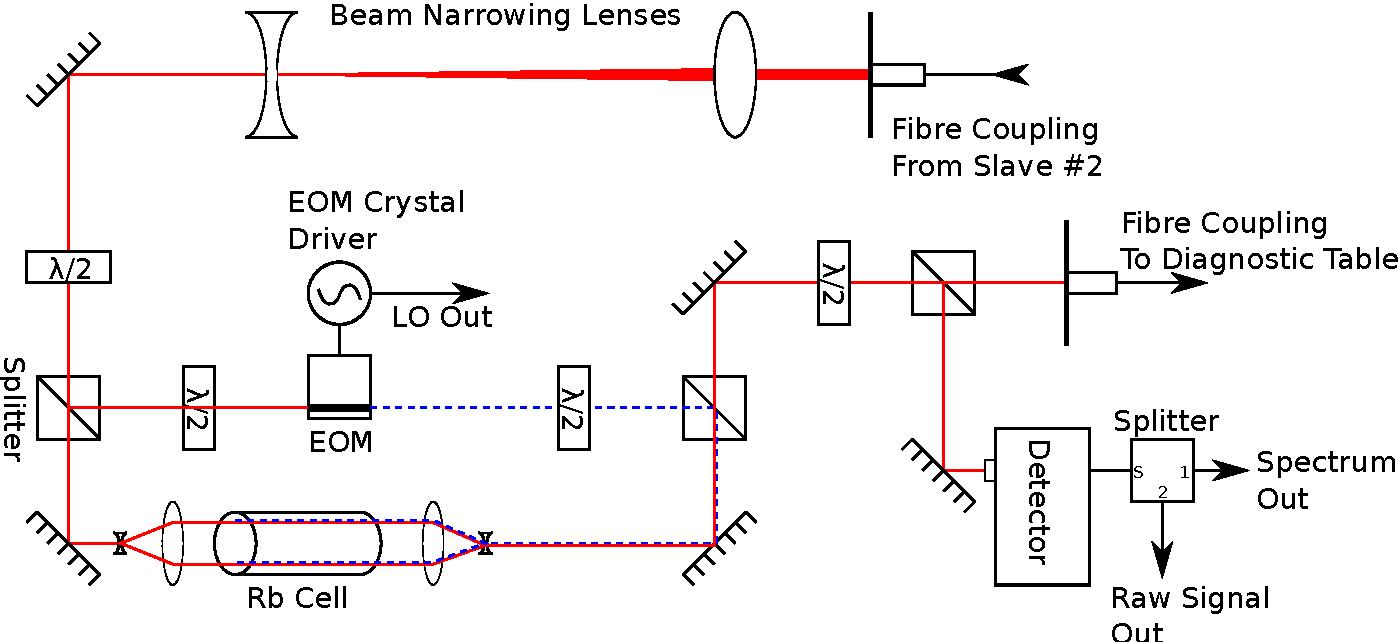
\includegraphics[width=\textwidth]{figures/optics.pdf}
  \centering\caption{A schematic overview of the optical setup.}
  \label{optics}
\end{figure}

An photograph the optical setup is shown in Figure~\ref{optical_setup}.  A schematic view of the same setup is shown in Figure~\ref{optics}.

    \subsubsection{Beam Focusing}
    %============================

The beam that comes out of the fibre coupler spreads too wide over the optical path of the feedback loop.  Thus, a telescope system was installed on the input fiber to reduce the size. A convex lens focusses the beam down, and a concave lens straightens the beam. By moving one of the lenses, the divergence can also be adjusted. This setup was calibrated to have a visibly collimated optical path length of about 2--3 metres. \\

    \subsubsection{Power Control}
    %============================

In several parts of the system, require precise control of beam power.  Specifically, this is needed in three locations: \\

\begin{enumerate}
    \item The power of the pump beam.
    \item The power of the probe beam.
    \item The power distribution between the diagnostic table and the detector.  The detector was visibly saturating in some tests, so this final stage is necessary.  It also makes diagnostics easier if a wide range of power can be arbitrarily redirected to the diagnostic table.
\end{enumerate}

In each of these locations, there is a half-wave plate followed by a pol cube.  The half wave plate rotates the polarization of linear polarized light.  The pol cube allows horizontally polarized light to pass straight through, while reflecting vertically polarized light\footnote{The pol cube does not work with 100\% efficiency—some horizontally polarized light will reflect and some vertically polarized light will pass straight through. This is commonly referred to as the `extinction ratio' and it puts a lower limit on the power levels in a given path}. \\

    \subsubsection{EOM and Crystal Driver}
    %===================================

\begin{figure}
  \includegraphics[width=.5\textwidth]{figures/eom_driver.jpg}
  \centering\caption{The EOM Crystal Driver circuit used.  The attenuation and phase adjustment potentiometers are visible.  Also visible, the output port (to EOM) and the ref output port (to LO).}
  \label{eom_driver}
\end{figure}

An EOM crystal driver was borrowed from the Phys 408 Optics lab.  It is shown in Figure~\ref{eom_driver}.  The availability of a working device greatly reduced the cost overhead of this project.  The driver generates a sinusoidal signal at approximately 20MHz, and is tuned to drive the high capacitance of the EOM crystal at a high voltage.  It also feeds out a reference to its internal oscillator.  This signal provides the local oscillator input for demodulation. \\

The EOM driver also includes a phase shift potentiometer to account for phase shifts that may occur in electrical lines or the optical path.  However, the shift provided by this potentiometer is woefully inadequate, with an approximate range of $\lambda/6$ (at least $\lambda/2$ would be ideal).  A phase delay was manually introduced using BNC cables of various lengths.  Of the cables tried, a 1.5m cable provided the best signal (but this method is clearly suboptimal).  The maximum phase shift of the driver is shown in Figure~\ref{fig:eom_phase}. \\

The light passing into the EOM must be horizontally polarized, thus a half-wave plate is used to re-polarize the light before it enters the EOM. \\

\begin{figure}
  \begin{tabular}{cc}
    \includegraphics[width=0.47\textwidth]{figures/{eom_driver_onboard_1}.jpg} &
    \includegraphics[width=0.47\textwidth]{figures/{eom_driver_onboard_2}.jpg} \\
  \end{tabular}
  \caption{The maximum phase shift of the EOM driver reference output, with no load attached.  Red signal corresponds to the driver (1MΩ), blue signal corresponds to LO out.  The impedance of the load affects the shape of both waveforms.}
  \label{fig:eom_phase}
\end{figure}

    \subsubsection{Pump Probe Modulation Transfer}
    %=============================================

The an EOM-modulated beam is fed into the sample from one direction (the \emph{pump} beam).  A single frequency beam (from the slave laser) passes through the gas in the opposite direction (the \emph{probe} beam).  Due to nonlinear interactions in the gas, the probe beam becomes modulated at the driving frequency of the pump beam.  That is, the pump beam modulates the gas, which in turn, modulates the probe beam. \\

The physics of the interaction between the two beams and the gas are described further in the \textbf{Section \ref{sec:theory}}. \\

Note that the cell has been installed at a slight angle, to minimize reflections off the surface of the cell. \\

    \subsubsection{Rb Cell Beam Expander}
    %====================================

The Rb gas cell has been surrounded in telescoping lenses to expand both the probe and pump beam.  This improves the signal-to-noise ratio by passing the beam through a larger fraction of the gas in the cell.  The telescopes increase the diameter of both beams by a factor of 3. \\

    \subsubsection{Heated Rb Cell}
    %=============================

Heating the rubidium cell can improve the signal to noise of this system.  At room temperature, a fraction of the rubidium in the cell exists as a solid on the surface of the cell.  By heating the cell, more rubidium will vapourize, increasing the density of the gas.  This causes the laser to pass through more gas, which strengthens the signal. \\

However, this effect cannot be used to arbitrary temperatures.  Increasing the temperature increase the vapour pressure, but it also increases the speed of the gas molecules, which causes the Doppler broadening to become worse, until the response ultimately becomes flat.  This effect is known as pressure broadening, and puts an upper limit on the possible performance improvements. \\

Heating was done with a pre-built heating coil and a measured with a K-type thermocouple.  For each temperature measurement, the heater was activated, and it's current load was manually adjusted the current output until the temperature reading on the thermocouple had remained stable for five minutes.  At the point of sampling, the heater was shut off (to eliminate any magnetic fields created by the current), and a measurement of the error signal was taken. \\

    \subsubsection{Cavity Wave Detector}
    %===================================

\begin{figure}
  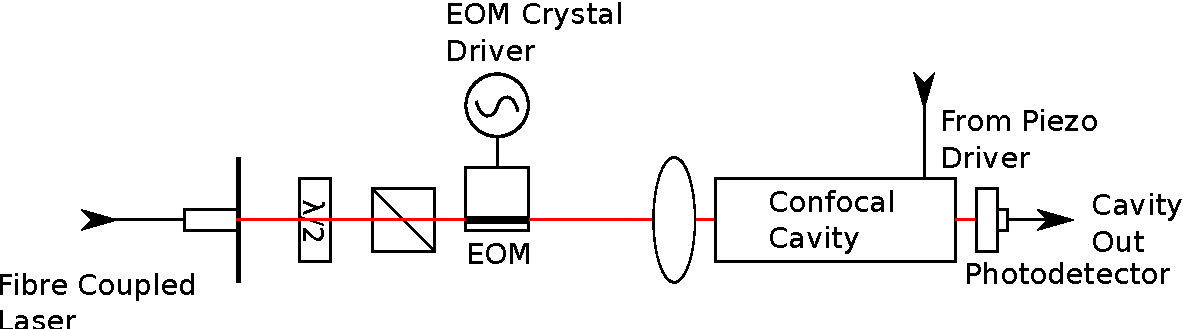
\includegraphics[width=\textwidth]{figures/cavity.pdf}
  \caption{Confocal cavity test setup.  The EOM is passed through a half wave plate, which allows us to adjust its polarization, and then through a pol cube which removes any vertically polarized light, leaving only horizontally polarized light.  The piezo element is fed by a function generator, and the piezo driving force, which corresponds to frequency, is plotted against the response of the photodetector.}
  \label{cavity}
\end{figure}

A confocal cavity was used to measure the effect the EOM has on the beam, to ensure that sidebands are in fact being created.  The setup of this cavity is shown in Figure~\ref{cavity}  The cavity resonates more highly with laser light that fits in an integer number of wavelengths within the cavity.  Having a photodiode on the end allows for measurement of the resonance amplitude.  The backside of the cavity can be moved by adjusting the voltage applied to a piezo system.  By feeding a triangular wave in (from a function generator), the (rough) frequency spectrum of the beam is observed. \\


\begin{figure}
  \centering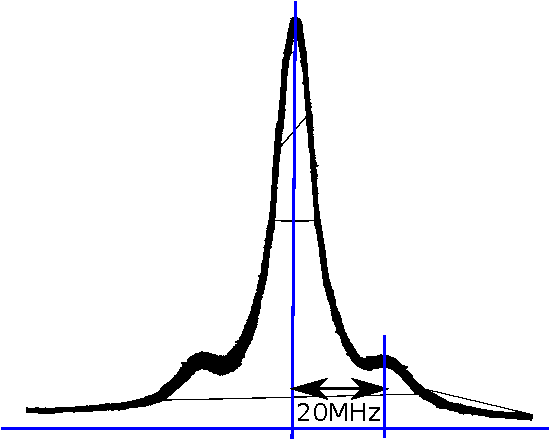
\includegraphics[width=0.5\textwidth]{figures/eom_wave.pdf}
  \caption{EOM Spectrum as viewed from the detector of a confocal cavity.  Sidebands appear on the light wave at ±20MHz from the carrier (which was calibrated from the free spectral range of the cavity). The measured sideband amplitudes were $14\pm1$\% of the carrier, which is approximately a 1:7:1 split of total power.}
  \label{fig:eom_wave}
\end{figure}

Figure~\ref{fig:eom_wave} shows that the EOM driver is functioning correctly. \\

    \subsubsection{Modulation Transfer Reference}
    %============================================

Since the frequency was sweept during the main tests, the low-frequency (near DC) part of the signal was isolated to give an indication of the actual modulation transfer spectrum.  This provided a continuous reference of which part of the spectrum was being sampled at all times. Additionally, this indicated how well the modulation transfer was working. \\

The raw signal itself, which we send off to the signal conditioning box, which converts it into a usable error signal. \\

\subsection{Signal Conditioning}
\label{sec:signalcond}

\begin{figure}
  \centering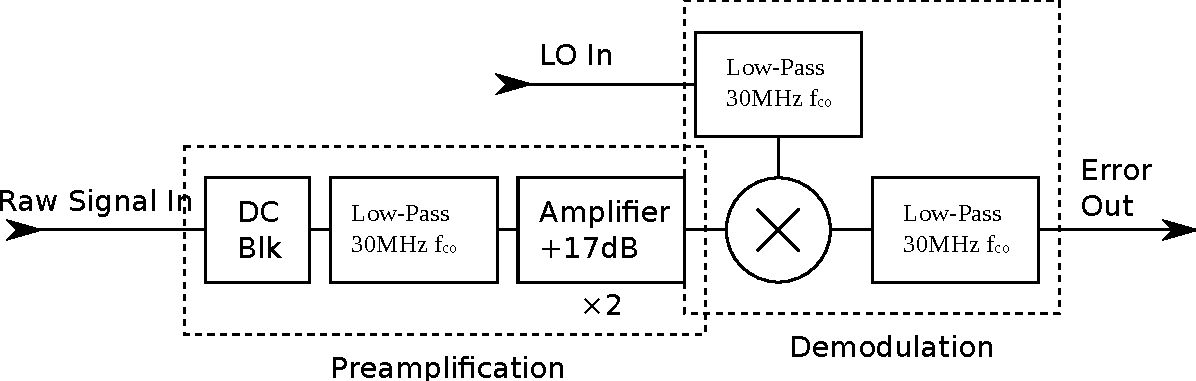
\includegraphics[width=\textwidth]{figures/rf_design.pdf}
  \caption{An overview of the signal conditioning stages.}
  \label{rf_design}
\end{figure}

An overview of the signal conditioning stages is shown in Figure~\ref{rf_design}. \\

    \subsubsection{Preamplification}
    %===============================

The 20MHz signal created at the detector is first filtered.  The DC component and everything above 30MHz are cut out, leaving ideally just the desired 20MHz signal.  That signal gets passed through two 17dB minicircuits RF amplifiers, which increase the power level of the signal enough to make it usable.  Each amplifier degrades the signal-to-noise by 6dB, so excessive chaining amplifiers should be avoided if possible. \\

    \subsubsection{Demodulation}
    %===========================

The preamplified signal is passed into a frequency mixer.  That signal is mixed with the 20MHz local oscillator (the EOM driver).  This gives us a desired signal at DC.  The mixed signal is then filtered at 10MHz, which eliminates any unwanted high frequency components.  The selection of frequency is important at this stage.  The higher a the cutoff frequency, the faster the system can respond to changes in the laser's frequency. However, setting a high frequency incurs a noise penalty.  The noise spread is linear, thus a doubling of frequency range decreases the SNR by 3dB. \\

A 10MHz cutoff frequency was chosen, primarily to eliminate known nonlinear artifacts of the mixer present at 20MHz; these filters reduce a signal at $2f_{co}$ by 40dB\cite{zfl_1000}.  Reducing this cutoff would further reduce the output noise. \\

\subsection{Infrastructure}
    \subsubsection{EOM Power Supply}
    %===============================

The homebuilt EOM driver CCA came with its own AC to DC converter.  However, supply noise proved to be a problem, so a custom power supply was developed for this board.  The power supply takes filtered DC lab power, and linearly downregulates to the needed input power. \\

    \subsubsection{Signal Conditioner Case and Power Distribution}
    %=============================================================

A custom case was built to contain the signal conditioning components.  It also includes a linear regulator which is capable of powering up to 4 of the minicircuits amplifiers.



%%%%%%%%%%%%%%%% IMPLEMENTATION

\newpage
\section{Validation}
\label{sec:validation}

\subsection{Data Collection}

Characteristic error signals were acquired for the Rb85 D2 $\left|F=3\right\rangle \rightarrow F'$ and Rb87 D2 $\left|F=2\right\rangle \rightarrow F'$ spectra for a variety of power/temperature combinations. For each spectrum, variable pump/probe power combinations were measured at room temperature. This is shown in \textbf{Appendix \ref{app:85pwr}, \ref{app:87pwr}}. From these sets, a power combination with a high SNR and large locking point slope was chosen to measure the effect of heating. As data processing was not performed until later, the best choice at the time was thought to be 4.0 mW for both pump and probe power. At these power levels the temperature was varied up to $\sim 100^\circ$ C, shown in \textbf{Appendix \ref{app:85temp}, \ref{app:87temp}}. It is clear from the data that the optimal temperature, with respect to slope/noise tradeoff, is likely between $20-40^\circ$ C and that the pressure broadening rapidly deteriorates the signal past $60^\circ$ C. \\

The SNR of the higher quality error signals is approximately 5:1 (e.g. 4.0 mW, 6.0 mW probe series). Though this seems poor compared to the existing AOM solution ($\sim$10:1), it is thought to mostly be a result of suboptimal electrical components. Simple improvements that can increase SNR by a factor of four or higher are suggested in \textbf{Section \ref{sec:recommendations}}.

\subsection{Locking Features}

Finding the desired locking point features first involved establishing a MHz/s scale on each of the time-domain spectra collected by the oscilloscope. All data sets were normalized to the reference AOM saturated absorption spectrum which was constant for each transition throughout data acquisition. This background spectrum was passed through a Savitzky-Golay piecewise polynomial filter to remove the higher frequency noise. Then, the two most prominent peaks correspond to the $\left|F=2\right\rangle \rightarrow F'=2,3$ and  $\left|F=2\right\rangle \rightarrow F'=1,3$ crossover resonances in Rb87 and the $\left|F=3\right\rangle \rightarrow F'=3,4$ and  $\left|F=3\right\rangle \rightarrow F'=2,4$ crossover resonances in Rb85.  The values of these resonances are known to high precision \cite{steckrb85, steckrb87}. Using their location, one can convert from the time domain to the frequency domain. \\

There are two primary sources of error in establishing these MHz/s scales. First, the peak-finding filter will have some error associated with it. As this is a piecewise interpolant and not a regression fit, it is difficult to specify quantitative value for the fit error, except by visual inspection. The second source of error is the laser ramping itself. The ramping signal for the laser servo is a low noise, nearly ideal triangle wave. However, the actual frequency response of the laser is not linear with respect to this ramp. The actual frequency of the laser will oscillate about the ramp, as per typical control system responses, thereby shrinking and stretching the frequency scale all across the data sets. The stated error in the frequency domain is a simple quadrature error that uses the standard deviation of the fit as a parameter. The sponsor is in agreement that this is a sufficient metric. \\

Questions were raised about the locations of the resonances across the data sets, and whether they moved in an obvious pattern as the pump:probe power ratios were changed. The locations of the modulation transfer spectrum peaks were acquired by applying a Savitzky-Golay filter to the modulation transfer spectrum and locating the extrema. As can be seen in \textbf{Figure \ref{fig:peak_drift}}, their measured location changes with no perceivable pattern. Furthermore, all of the data points are within each other's error bars in the frequency domain, and can therefore be considered static. \\

The slope and noise about the optimal locking points in each spectrum were derived by a simple linear regression in a small window about the resonance peaks. The fitted line was subtracted from the data and the min/max of the resultant signal in that same window was used to determine the noise in mVpp. It may be prudent to instead compute RMS noise in the window, but, upon visual inspection, the background noise signal was consistent in amplitude across the spectrum, and so they are likely to be closely related by the $\sqrt{2}$ ratio of an ideal, monochromatic sinusoid. Given the data for the 6.0 mW:6.0 mW data sets, the resulting frequency domain noise about these points is expected to be $\sim$4.52 MHz-pp for Rb87 and $\sim$3.82 MHz-pp for Rb85. Comparively, the AOM data shown in \textbf{Figure \ref{fig:aom_spectra}} yields $\sim$0.88 MHz-pp for Rb87 and $\sim$0.46 MHz-pp for Rb85. It is not easy to determine what effective laser linewidth this would result in for a laser that is locking to the null point, rather than being swept. Additionally, the AOM data is filtered down to approximately 10 kHz, and while the SNR is high, it is difficult to tell how this bandwidth limitation would affect the laser servo. Additionally, making the proposed component improvements would bring the new system's frequency noise down by a factor of four, at minimum, putting it on-par with the AOM system, without the bandwidth limitations.

\begin{figure}
  \begin{tabular}{cc}
    \includegraphics[width=0.47\textwidth]{figures/{85_peak_drift}.png} &
    \includegraphics[width=0.47\textwidth]{figures/{87_peak_drift}.png} \\
  \end{tabular}
  \caption[Modulation transfer, locking point drift]{ Behaviour of modulation transfer peaks as a function of varying probe/pump power. Only the three most prominent peaks were consistently resolvable. The error is calculated from the scale fitting variance, and increases for higher frequency regions.}
  \label{fig:peak_drift}
\end{figure}


%%%%%%%%%%%%%%%% DELIVERABLES

\newpage
\section{Project Deliverables}

\subsection{EOM-based Optical Setup}

The sponsor's requirement of an optical pipeline including an EOM unit, Rubidium vapour cell and photosensor coupling was fully met. Due to the difficulty of creating a precise optical pipeline, it was decided to pursuse existing home-built or pre-built solutions whenever possible. The component and implementation specifics are discussed in further detail in \textbf{Section \ref{sec:implementation}}.

\subsection{Fast Analog Feedback Circuit}

The feedback circuit was built around a single channel demodulation path using discrete RF components and the EOM driver's reference output. The component and implementation specifics are discussed in further detail in \textbf{Section \ref{sec:signalcond}}. The specific RF components used for signal processing are detailed in \textbf{Appendix \ref{app:components}}.

\subsection{New vs. Old System Characterization}

Originally, the sponsor had suggested closed-loop testing of this locking scheme. With the use of a Fabry-P{\'e}rot interferometer, a direct comparison of laser linewidths using the old and new locking systems could be made. Unfortunately, due to timing, it was not possible to access, and make large changes to, the master laser table when this new system neared completion. During development, Madison Group researchers began experimental procedures which could not be easily interrupted. Additionally, it would have been either time-consuming or suboptimal to route either the relevant optical or electrical signals across the room from this optical table to the laser servo racks. The sponsor, Dr. Kirk Madison, instead directed testing to acquire broad error signal metrics including:
\begin{itemize}
    \item Error signals with variable pump/probe power
    \item Error signals with fixed pump/probe power and variable temperature
\end{itemize}
and, critically, the slope (mV/MHz) and noise (mVpp) around the main locking points. It is intended that Madison Group researchers use this data to rebuild this setup on the master laser optical table at their convenience. This data is shown in \textbf{Appendices \ref{app:85pwr} - \ref{app:87temp}}. The methods used to generate the data are discussed in \textbf{Section \ref{sec:validation}}.

%%%%%%%%%%%%%%%% RECOMMENDATIONS

\newpage

\section{Recommendations}
\label{sec:recommendations}

\subsection{Improved Phase Adjustment}

Current understanding of modulation transfer spectroscopy indicates that the position of the zero crossing is independant of the phase adjustment.  However, as shown in prior work, the amplitude of the signal is not \cite{0957-0233-19-10-105601}. The onboard phase adjustment is limiting in its range, as shown in \textbf{Figure \ref{fig:eom_phase}}.  Implementing an improved phase adjustment which allows a full $\lambda/2$ would make this optimization much easier to do.

\subsection{EOM driving frequencies}

The features in the Rb85 transitions are roughly 30 MHz apart.  With a 20 MHz EOM driver signal, it was noticed that the fringes of two strong signals overlap, crossing zero at a crossover.  If a 30 MHz EOM driver were used instead, these two signals might constructively amplify, creating a very clean error signal. Since the EOM driver oscillator frequency was non-adjustable, it was not possible to characterize its effect on the error signal.

\subsection{Laser Power}

The highest quality error signal obtained made used 100\% of available laser power.  It is possible that by increasing the power even further, an even-better signal-to-noise ratio could be achieved.

\subsection{Improved pre-amplifiers}

The most obvious path to noise improvement is selecting better amplifiers.  The amplifiers used here, MiniCircuits ZFL-1000+, also exists in a low noise variant, the ZFL-1000LN+.  This amplifier has nearly identical properties, but the noise figure is lower, 3dB instead of 6dB \footnote{Noise figure is the amount that the SNR is increased by the amplifier.  Given a -20 dBm carrier, with -30 dBm of noise, and a +20 dB amplifier with +6 dB noise figure, the output signal will contain a 0dBm carrier, and -14dBm of noise, changing the SNR from 10 dB to 4 dB.}. The best locking features in \textbf{Appendices \ref{app:85pwr} - \ref{app:87temp}} have an SNR of approximately 5:1. The existing AOM signal (\textbf{Figure \ref{fig:aom_spectra}}), has an SNR of approximately 10:1. Switching out the existing amplifiers for a better model should increase the SNR by 6 dB, to a value of 20:1 (two amplifiers in series). This is more robust than the existing AOM solution. \\

Additionally, the amplifiers used do not have the desired specifications.  They are the most appropriate choice given the supplier (Mini-Circuits), but they are over-specified.  These amplifiers are designed to work up to 1000 MHz, whereas an ideal cutoff would be in the range of 25-30 MHz.  There are likely amplifiers better suited to this purpose.  If not, then one could probably be made which meets these specifications, and has very good performance.  See, for example TI's guide to RF op amp circuits.\cite{ti_amps}.

\subsection{Additional Low-Pass Filtering}

A spectral analysis of the noise indicates that the energy distribution is flat in frequency, white noise, up to the low-pass cutoff frequency (10 MHz).  A crude, but likely effective way to remove noise would be to bring in a lower low-pass filter, which would have the effect of `averaging' the error signal in time, reducing the amount of white noise, at the cost of response time.


\subsection{Closed Loop Operation}

In order for the system to actually be used, the feedback loop would need to be closed.  That is, the demodulated error signal would need to be fed back into a laser diode controller, which would use the signal to adjust the frequency of the laser itself.  A suitable solution available in the lab was the Vescent D2-105 laser controller, which includes fast (current) and slow (piezo) control, and a built in PI$^2$D controller.  This was not implemented, as the sponsor indicated that they would prefer a deeper investigation of possible tactics to improve the error signal, versus closing the loop and providing a functional (but sub-optimal) solution.



%%%%%%%%%%%%%%%% CONCLUSION

\newpage
\section{Conclusion}

The feedback system built here, based around an EOM and modulation transfer spectroscopy, provides the Madison Group researchers with a more robust method of precisely locking a laser to an atomic transition resonance of rubidium. \\

Construction was completed on a optical table setup based around a rubidium vapour cell, and a Pound-Drever-Hall type error signal was generated using a photosensor and discrete RF components. Optical modulation was achieved with an existing home-built EOM with a Lithium Niobiate crystal and corresponding driving electronics.\\

The new system offers a signal bandwidth of 10 MHz, though this can be pushed closer to the EOM modulation frequency with better filter solutions. It was shown that the locking points are stable, and that their resultant frequency domain noise is comparable with the existing AOM system, assuming identical laser servo behaviour. Though the SNR in the data sets is lower than desired, it can easily be improved by a signifcant margin, further reducing the frequency domain noise. Substituting suboptimal electrical components will increase SNR by a factor of four, at minimum. Signal averaging can also improve this significantly, but at a cost of bandwidth.

\section*{Acknowledgements}
\addcontentsline{toc}{section}{Acknowledgements}

This project was aided immensely by the research staff in the UBC Quantum Degenerate Gases laboratory led by Dr. Kirk Madison. Dr. Madison provided direct guidence on theoretical matters and contributed significant physical resources. Gene Polovy and Will Gunton of the Madison Group were extremely helpful with the physical setup, and with locating equipment. Janelle van Dongen provided significant assistance with the laser control instrumentation and data acquisition. Further thanks goes to Dr. David Jones, Dr. Jim Booth, Mariusz Semczuk, Koko Yu, Kahan Dare and Kais Jooya for their suggestions and guidance.

%%%%%%%%%%%%%%%% APPENDICES

\newpage
\section*{Appendix}
\addcontentsline{toc}{section}{Appendix}
\renewcommand{\thesubsection}{\Alph{subsection}}

\subsection{Rb85 Error Signals - Variable Power}
\label{app:85pwr}
%
%   0.5mW Probe
%
\begin{figure}[H]
  \begin{tabular}{cc}
    \includegraphics[width=0.47\textwidth]{figures/{85_0.5mW_1.0mW}.png} &
    \includegraphics[width=0.47\textwidth]{figures/{85_0.5mW_2.0mW}.png} \\
    (a) Probe:Pump 0.5:1.0 (mW) & (b) Probe:Pump 0.5:2.0 (mW) \\[6pt]
    \includegraphics[width=0.47\textwidth]{figures/{85_0.5mW_4.0mW}.png} &
    \includegraphics[width=0.47\textwidth]{figures/{85_0.5mW_10.5mW}.png} \\
    (c) Probe:Pump 0.5:4.0 (mW) & (d) Probe:Pump 0.5:10.5 (mW) \\[6pt]
  \end{tabular}
  \caption{Modulation transfer spectroscopy error signals near the Rb85 $\left|F=3\right\rangle$ with 0.5 mW probe power and variable pump power. Each figure shows the AOM-derived reference spectrum (black), the EOM-based modulation transfer spectrum (blue) and the resulting PDH error signal (red). Measured 1/e beam diameters inside the cell are approximately 4.0 mm for both beams.}
\end{figure}
\newpage
%
%   1.0mW Probe
%
\begin{figure}[H]
  \begin{tabular}{cc}
    \includegraphics[width=0.47\textwidth]{figures/{85_1.0mW_1.0mW}.png} &
    \includegraphics[width=0.47\textwidth]{figures/{85_1.0mW_2.0mW}.png} \\
    (a) Probe:Pump 1.0:1.0 (mW) & (b) Probe:Pump 1.0:2.0 (mW) \\[6pt]
    \includegraphics[width=0.47\textwidth]{figures/{85_1.0mW_4.0mW}.png} &
    \includegraphics[width=0.47\textwidth]{figures/{85_1.0mW_10.1mW}.png} \\
    (c) Probe:Pump 1.0:4.0 (mW) & (d) Probe:Pump 1.0:10.1 (mW) \\[6pt]
  \end{tabular}
  \caption{Modulation transfer spectroscopy error signals near the Rb85 $\left|F=3\right\rangle$ transitions with 1.0 mW probe power and variable pump power. Each figure shows the AOM-derived reference spectrum (black), the EOM-based modulation transfer spectrum (blue) and the resulting PDH error signal (red). Measured 1/e beam diameters inside the cell are approximately 4.0 mm for both beams.}
\end{figure}
\newpage
%
%   2.0mW Probe
%
\begin{figure}[H]
  \begin{tabular}{cc}
    \includegraphics[width=0.47\textwidth]{figures/{85_2.0mW_1.0mW}.png} &
    \includegraphics[width=0.47\textwidth]{figures/{85_2.0mW_2.0mW}.png} \\
    (a) Probe:Pump 2.0:1.0 (mW) & (b) Probe:Pump 2.0:2.0 (mW) \\[6pt]
    \includegraphics[width=0.47\textwidth]{figures/{85_2.0mW_4.0mW}.png} &
    \includegraphics[width=0.47\textwidth]{figures/{85_2.0mW_9.3mW}.png} \\
    (c) Probe:Pump 2.0:4.0 (mW) & (d) Probe:Pump 2.0:9.3 (mW) \\[6pt]
  \end{tabular}
  \caption{Modulation transfer spectroscopy error signals near the Rb85 $\left|F=3\right\rangle$ transitions with 2.0 mW probe power and variable pump power. Each figure shows the AOM-derived reference spectrum (black), the EOM-based modulation transfer spectrum (blue) and the resulting PDH error signal (red). Measured 1/e beam diameters inside the cell are approximately 4.0 mm for both beams.}
\end{figure}
\newpage
%
%   4.0mW Probe
%
\begin{figure}[H]
  \begin{tabular}{cc}
    \includegraphics[width=0.47\textwidth]{figures/{85_4.0mW_1.0mW}.png} &
    \includegraphics[width=0.47\textwidth]{figures/{85_4.0mW_2.0mW}.png} \\
    (a) Probe:Pump 4.0:1.0 (mW) & (b) Probe:Pump 4.0:2.0 (mW) \\[6pt]
    \includegraphics[width=0.47\textwidth]{figures/{85_4.0mW_4.0mW}.png} &
    \includegraphics[width=0.47\textwidth]{figures/{85_4.0mW_7.7mW}.png} \\
    (c) Probe:Pump 4.0:4.0 (mW) & (d) Probe:Pump 4.0:7.7 (mW) \\[6pt]
  \end{tabular}
  \caption{Modulation transfer spectroscopy error signals near the Rb85 $\left|F=3\right\rangle$ transitions with 4.0 mW probe power and variable pump power. Measured 1/e beam diameters inside the cell are approximately 4.0 mm for both beams.}
\end{figure}
\newpage
%
%   6.0mW Probe
%
\begin{figure}[H]
  \begin{tabular}{cc}
    \includegraphics[width=0.47\textwidth]{figures/{85_6.0mW_1.0mW}.png} &
    \includegraphics[width=0.47\textwidth]{figures/{85_6.0mW_2.0mW}.png} \\
    (a) Probe:Pump 6.0:1.0 (mW) & (b) Probe:Pump 6.0:2.0 (mW) \\[6pt]
    \includegraphics[width=0.47\textwidth]{figures/{85_6.0mW_4.0mW}.png} &
    \includegraphics[width=0.47\textwidth]{figures/{85_6.0mW_6.0mW}.png} \\
    (c) Probe:Pump 6.0:4.0 (mW) & (d) Probe:Pump 6.0:6.0 (mW) \\[6pt]
  \end{tabular}
  \caption{Modulation transfer spectroscopy error signals near the Rb85 $\left|F=3\right\rangle$ transitions with 6.0 mW probe power and variable pump power. Each figure shows the AOM-derived reference spectrum (black), the EOM-based modulation transfer spectrum (blue) and the resulting PDH error signal (red). Measured 1/e beam diameters inside the cell are approximately 4.0 mm for both beams.}
\end{figure}
\newpage

\subsection{Rb85 Error Signals - Variable Temperature}
\label{app:85temp}

\begin{figure}[H]
  \begin{tabular}{cc}
    \multicolumn{2}{c}{\includegraphics[width=0.47\textwidth]
    {figures/{85_4.0mW_4.0mW}.png} }\\
    \multicolumn{2}{c}{(a) 22$^{\circ}$ C } \\[10pt]
    \includegraphics[width=0.47\textwidth]{figures/{85_40C}.png} &
    \includegraphics[width=0.47\textwidth]{figures/{85_60C}.png} \\
    (b) 40$^{\circ}$ C & (c) 60$^{\circ}$ C  \\[6pt]
    \includegraphics[width=0.47\textwidth]{figures/{85_80C}.png} &
    \includegraphics[width=0.47\textwidth]{figures/{85_102C}.png} \\
    (d) 80$^{\circ}$ C  & (e) 102$^{\circ}$ C  \\[6pt]
  \end{tabular}
  \caption{Modulation transfer spectroscopy error near the Rb87 $\left|F=2\right\rangle$ transitions with varying temperature. Each figure shows the AOM-derived reference spectrum (black), the EOM-based modulation transfer spectrum (blue) and the resulting PDH error signal (red). Pump and probe beam power were both held at a constant 4.0 mW. Measured 1/e beam diameters inside the cell are approximately 4.0 mm for both beams. Past 60$^{\circ}$, the spectrum rapidly beacame unusable due to pressure broadening. The 22$^{\circ}$ C data is included again for easy reference.}
\end{figure}
\newpage

\subsection{Rb87 Error Signals - Variable Power}
\label{app:87pwr}
%
%   0.5mW Probe
%
\begin{figure}[H]
  \begin{tabular}{cc}
    \includegraphics[width=0.47\textwidth]{figures/{87_0.5mW_1.0mW}.png} &
    \includegraphics[width=0.47\textwidth]{figures/{87_0.5mW_2.0mW}.png} \\
    (a) Probe:Pump 0.5:1.0 (mW) & (b) Probe:Pump 0.5:2.0 (mW) \\[6pt]
    \includegraphics[width=0.47\textwidth]{figures/{87_0.5mW_4.0mW}.png} &
    \includegraphics[width=0.47\textwidth]{figures/{87_0.5mW_10.4mW}.png} \\
    (c) Probe:Pump 0.5:4.0 (mW) & (d) Probe:Pump 0.5:10.4 (mW) \\[6pt]
  \end{tabular}
  \caption{Modulation transfer spectroscopy error signals near the Rb87 $\left|F=2\right\rangle$ with 0.5 mW probe power and variable pump power. Each figure shows the AOM-derived reference spectrum (black), the EOM-based modulation transfer spectrum (blue) and the resulting PDH error signal (red). Measured 1/e beam diameters inside the cell are approximately 4.0 mm for both beams.}
\end{figure}
\newpage
%
%   1.0mW Probe
%
\begin{figure}[H]
  \begin{tabular}{cc}
    \includegraphics[width=0.47\textwidth]{figures/{87_1.0mW_1.0mW}.png} &
    \includegraphics[width=0.47\textwidth]{figures/{87_1.0mW_2.0mW}.png} \\
    (a) Probe:Pump 1.0:1.0 (mW) & (b) Probe:Pump 1.0:2.0 (mW) \\[6pt]
    \includegraphics[width=0.47\textwidth]{figures/{87_1.0mW_4.0mW}.png} &
    \includegraphics[width=0.47\textwidth]{figures/{87_1.0mW_9.9mW}.png} \\
    (c) Probe:Pump 1.0:4.0 (mW) & (d) Probe:Pump 1.0:9.9 (mW) \\[6pt]
  \end{tabular}
  \caption{Modulation transfer spectroscopy error signals near the Rb87 $\left|F=2\right\rangle$ transitions with 1.0 mW probe power and variable pump power. Each figure shows the AOM-derived reference spectrum (black), the EOM-based modulation transfer spectrum (blue) and the resulting PDH error signal (red). Measured 1/e beam diameters inside the cell are approximately 4.0 mm for both beams.}
\end{figure}
\newpage
%
%   2.0mW Probe
%
\begin{figure}[H]
  \begin{tabular}{cc}
    \includegraphics[width=0.47\textwidth]{figures/{87_2.0mW_1.0mW}.png} &
    \includegraphics[width=0.47\textwidth]{figures/{87_2.0mW_2.0mW}.png} \\
    (a) Probe:Pump 2.0:1.0 (mW) & (b) Probe:Pump 2.0:2.0 (mW) \\[6pt]
    \includegraphics[width=0.47\textwidth]{figures/{87_2.0mW_4.0mW}.png} &
    \includegraphics[width=0.47\textwidth]{figures/{87_2.0mW_9.3mW}.png} \\
    (c) Probe:Pump 2.0:4.0 (mW) & (d) Probe:Pump 2.0:9.3 (mW) \\[6pt]
  \end{tabular}
  \caption{Modulation transfer spectroscopy error signals near the Rb87 $\left|F=2\right\rangle$ transitions with 2.0 mW probe power and variable pump power. Each figure shows the AOM-derived reference spectrum (black), the EOM-based modulation transfer spectrum (blue) and the resulting PDH error signal (red). Measured 1/e beam diameters inside the cell are approximately 4.0 mm for both beams.}
\end{figure}
\newpage
%
%   4.0mW Probe
%
\begin{figure}[H]
  \begin{tabular}{cc}
    \includegraphics[width=0.47\textwidth]{figures/{87_4.0mW_1.0mW}.png} &
    \includegraphics[width=0.47\textwidth]{figures/{87_4.0mW_2.0mW}.png} \\
    (a) Probe:Pump 4.0:1.0 (mW) & (b) Probe:Pump 4.0:2.0 (mW) \\[6pt]
    \includegraphics[width=0.47\textwidth]{figures/{87_4.0mW_4.0mW}.png} &
    \includegraphics[width=0.47\textwidth]{figures/{87_4.0mW_7.6mW}.png} \\
    (c) Probe:Pump 4.0:4.0 (mW) & (d) Probe:Pump 4.0:7.6 (mW) \\[6pt]
  \end{tabular}
  \caption{Modulation transfer spectroscopy error signals near the Rb87 $\left|F=2\right\rangle$ transitions with 4.0 mW probe power and variable pump power. Each figure shows the AOM-derived reference spectrum (black), the EOM-based modulation transfer spectrum (blue) and the resulting PDH error signal (red). Measured 1/e beam diameters inside the cell are approximately 4.0 mm for both beams.}
\end{figure}
\newpage
%
%   6.0mW Probe
%
\begin{figure}[H]
  \begin{tabular}{cc}
    \includegraphics[width=0.47\textwidth]{figures/{87_6.0mW_1.0mW}.png} &
    \includegraphics[width=0.47\textwidth]{figures/{87_6.0mW_2.0mW}.png} \\
    (a) Probe:Pump 6.0:1.0 (mW) & (b) Probe:Pump 6.0:2.0 (mW) \\[6pt]
    \includegraphics[width=0.47\textwidth]{figures/{87_6.0mW_4.0mW}.png} &
    \includegraphics[width=0.47\textwidth]{figures/{87_6.0mW_5.8mW}.png} \\
    (c) Probe:Pump 6.0:4.0 (mW) & (d) Probe:Pump 6.0:5.8 (mW) \\[6pt]
  \end{tabular}
  \caption{Modulation transfer spectroscopy error signals near the Rb87 $\left|F=2\right\rangle$ transitions with 6.0 mW probe power and variable pump power. Each figure shows the AOM-derived reference spectrum (black), the EOM-based modulation transfer spectrum (blue) and the resulting PDH error signal (red). Measured 1/e beam diameters inside the cell are approxximately 4.0 mm for both beams.}
\end{figure}
\newpage

\subsection{Rb87 Error Signals - Variable Temperature}
\label{app:87temp}

\begin{figure}[H]
  \begin{tabular}{cc}
    \multicolumn{2}{c}{\includegraphics[width=0.47\textwidth]
    {figures/{87_4.0mW_4.0mW}.png} }\\
    \multicolumn{2}{c}{(a) 22$^{\circ}$ C } \\[10pt]
    \includegraphics[width=0.47\textwidth]{figures/{87_40C}.png} &
    \includegraphics[width=0.47\textwidth]{figures/{87_60C}.png} \\
    (b) 40$^{\circ}$ C & (c) 60$^{\circ}$ C  \\[6pt]
    \includegraphics[width=0.47\textwidth]{figures/{87_80C}.png} &
    \includegraphics[width=0.47\textwidth]{figures/{87_100C}.png} \\
    (d) 80$^{\circ}$ C  & (e) 100$^{\circ}$ C  \\[6pt]
  \end{tabular}
  \caption{Modulation transfer spectroscopy error near the Rb87 $\left|F=2\right\rangle$ transitions with varying temperature. Each figure shows the AOM-derived reference spectrum (black), the EOM-based modulation transfer spectrum (blue) and the resulting PDH error signal (red). Pump and probe beam power were both held at a constant 4.0 mW. Measured 1/e beam diameters inside the cell are approximately 4.0 mm for both beams. As with the Rb85 data, the spectrum rapidly beacame unusable past 60$^{\circ}$C due to pressure broadening. The 22$^{\circ}$ C data is included again for easy reference.}
\end{figure}
\newpage

\subsection{Electrical Components List}
\label{app:components}

\begin{table}[!hrt]
  \begin{tabularx}{\linewidth}{|L|L|L|}
  \hline
  \textbf{Item} & \textbf{MFPN} & \textbf{Approx. Purchase Cost} \\
  \hline
  DC Block & BLK-89+ & \$20 \\
  Broadband 1GHz Amplifier & ZFL-1000+ & \$70 \\
  LPF 30 MHz & SLP-30+ & \$30 \\
  LPF 10.7 MHz & SLP-10.7+ & \$30 \\
  Balanced RF Mixer & ZX05-1L-S+ & \$30 \\
  Passive Splitter/Combiner & ZFRSC-42-S+ & \$50 \\
  \hline
  \end{tabularx}
  \caption{Brief overview of discrete RF components used in generating the in-phase PDH error signal. All components were acquired from Mini-Circuits. A simple LDO circuit was built to convert QDG Lab power to the necessary voltage levels. Mini-circuits invoice: 2-QT-314867-B.}
  \label{budget_table}
\end{table}

%%%%%%%%%%%%%%%% REFERENCES

\newpage
\printbibliography

\end{document}



